\documentclass{beamer}

\usepackage[utf8]{inputenc}
\usepackage[spanish]{babel}
\usepackage[normalem]{ulem}
\usepackage{graphicx}

\usetheme{Rochester}
\usecolortheme{seagull}
\beamertemplatenavigationsymbolsempty

\title[Inflación y poder adquisitivo]{Inflación heterogénea\\y poder adquisitivo en Argentina}
\subtitle{Revisión de Fuentes}
\author{Javier Spina}
\institute{ECyT - UNSAM}
\date{8 de mayo de 2026}

\begin{document}

\begin{frame}
    \titlepage
\end{frame}


\section{Selección de Papers}
\begin{frame}{¿Dónde estábamos?}
    \begin{itemize}
        \item \textbf{Jaravel (2024)} --- \textit{Distributional Consumer Price Indices}\\
              \vspace{0.4em}
        \item \textbf{Lódola, Busso y Cerimedo (2000)} --- \textit{Sesgos en el IPC: el sesgo plutocrático en Argentina}\\
              \vspace{0.4em}
        \item \textbf{Deaton (1985)} --- \textit{Panel data from time series of cross-sections}\\
    \end{itemize}
\end{frame}

\begin{frame}{Scope, scope, scope}
\centering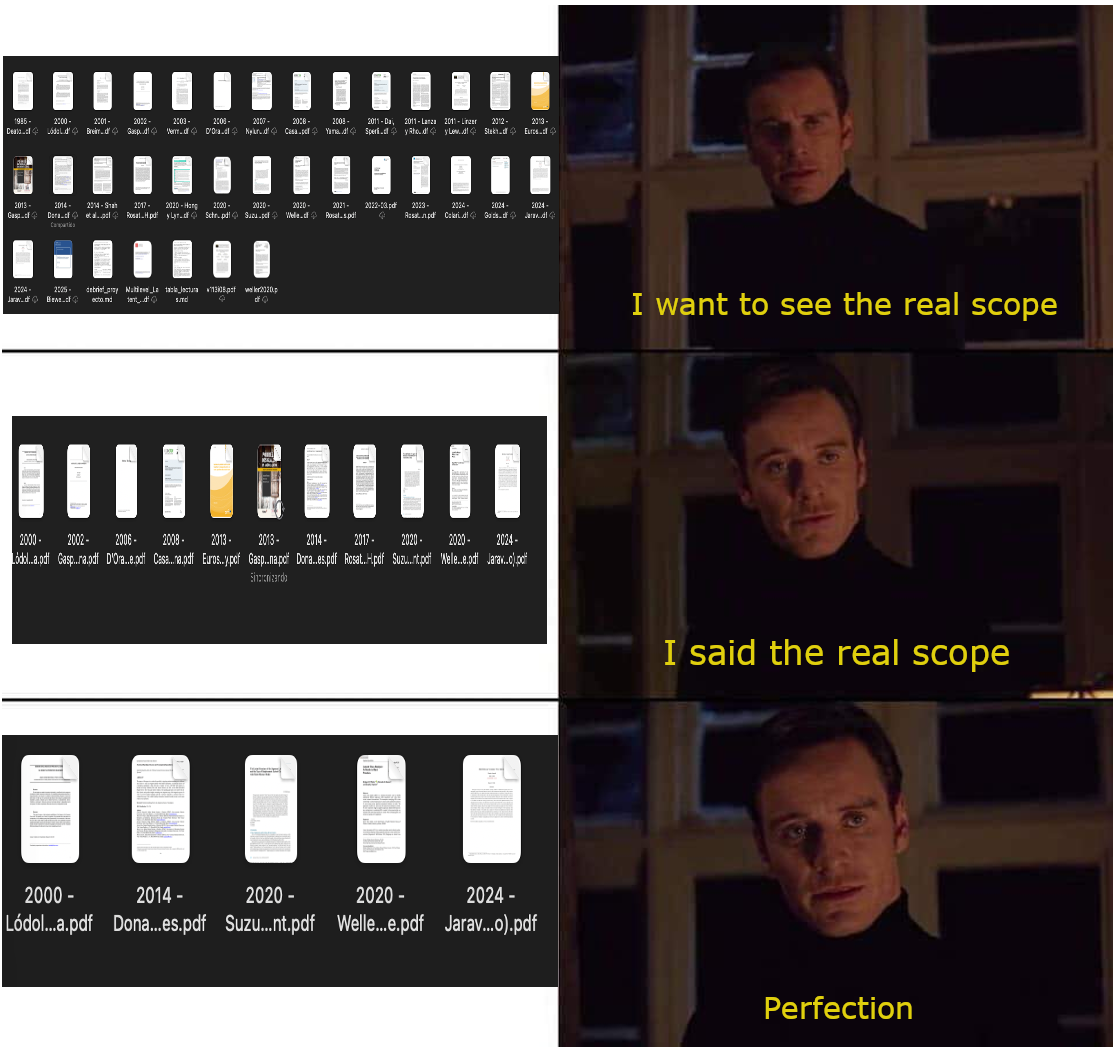
\includegraphics[height=0.95\textheight]{the_real_scope.png}
\end{frame}

\begin{frame}{Scope, scope, scope}
    \begin{itemize}
        \item \textbf{Jaravel (2024)} --- \textit{Distributional Consumer Price Indices}
              \vspace{0.4em}
        \item \textbf{Lódola, Busso y Cerimedo (2000)} --- \textit{Sesgos en el IPC: el sesgo plutocrático en Argentina}
              \vspace{0.4em}
        \item \sout{\textbf{Deaton (1985)} --- \textit{Panel data from time series of cross-sections}}
    \end{itemize}
\end{frame}


\begin{frame}{Dos marcos teóricos}
    \begin{itemize}
        \item Ciencia de Datos
        \begin{itemize}
            \item \textbf{Suzuki (2020)} --- \textit{The Latent Structure of the Japanese Labor Market and the Type of Employment}
                \vspace{0.4em}
            \item \textbf{Donatiello et al (2014)} --- \textit{Statistical Matching of Income and Consumption Expenditures}
                \vspace{0.4em}
            \item \textbf{INDEC} --- \textit{Documentación técnica y diseño de registros}
                \vspace{0.4em}
            \item \textbf{Weller, Bowen y Faubert (2020)} --- \textit{Latent Class Analysis: A Guide to Best Practice}
                \vspace{0.8em}
        \end{itemize}
        \item Ciencias Económicas
        \begin{itemize}
            \item \textbf{Jaravel (2024)} --- \textit{Distributional Consumer Price Indices}
              \vspace{0.4em}
            \item \textbf{Lódola, Busso y Cerimedo (2000)} --- \textit{Sesgos en el IPC: el sesgo plutocrático en Argentina}
        \end{itemize}
    \end{itemize}
\end{frame}


\section{El dominio económico}
\begin{frame}{¿Por qué IPC heterogéneo?}
    % \begin{block}{Pregunta central}
    %     ¿Cuál es la tasa de inflación real que enfrenta cada perfil de trabajador argentino, y qué tan vulnerable es su situación cuando se mide con ese índice en lugar del IPC oficial?
    % \end{block}
    \begin{block}{¿Qué fuente habilita el uso de perfiles?}
        \textbf{Jaravel} sugiere que la inflación heterogénea puede ser estudiada más allá del corte clásico por deciles de ingreso. De hecho, usa grupos etarios, grupos étnicos, geografía, características del hogar.
    \end{block}

    \begin{block}{Jaravel (2024), pp. 9-11}
        \textit{``This approach can be applied to any socio-demographic group – by income, age, race, gender, occupations, etc.''}
    \end{block}
    \begin{block}{Lódola, Busso y Cerimedo (2000), p. 1}
        \textit{``Esta cuestión [que la inflación no refleje el impacto real en algunos consumidores] se relaciona con si debe existir índices de precios para diferentes grupo, por ejemplo: ancianos y no ancianos, urbanos y rurales, ricos y pobres.''}
    \end{block}
\end{frame}

\section{Propuestas de Ciencia de Datos}
\begin{frame}{El aporte de la Ciencia de Datos}
    \begin{itemize}
        \item Introducir mediante técnicas de aprendizaje automático una manera de distinguir estructuras latentes.
        \item Integrar bases puntuales (ENGHo) con bases continuas (EPH) para panelizar (o pseudo-panelizar) los perfiles encontrados.
     \end{itemize}
% insertar dos screenshots de los papers de Suzuki y Donatiello con dos minipages paralelos en vertical
    \begin{figure}
        \begin{minipage}{0.45\textwidth}
            \centering
            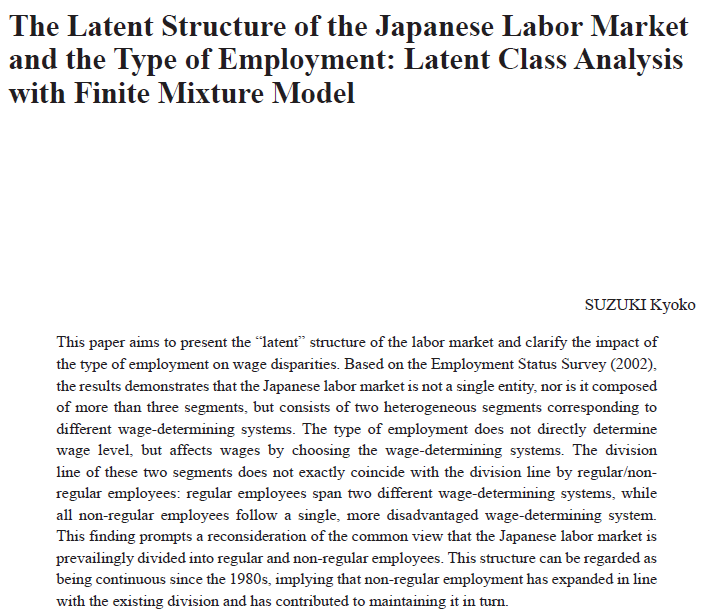
\includegraphics[width=\textwidth]{suzuki.png}
            % \caption{Suzuki (2020), p. 5}
        \end{minipage}\hfill
        \begin{minipage}{0.45\textwidth}
            \centering
            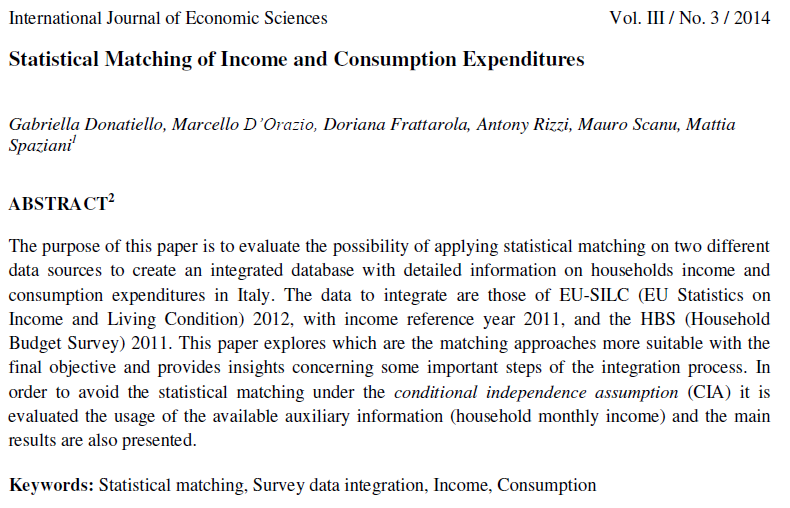
\includegraphics[width=\textwidth]{donatiello.png}
            % \caption{Donatiello et al (2014), p. 3}
        \end{minipage}
    \end{figure}
\end{frame}

\begin{frame}{La propuesta metodológica}
\centering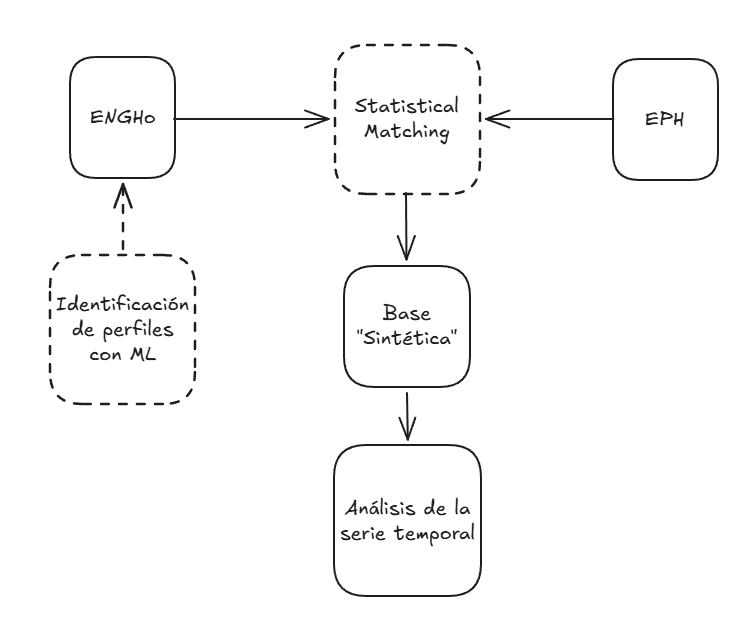
\includegraphics[width=0.8\textwidth]{pipeline.png}
\end{frame}

\begin{frame}{Los datos}
\begin{itemize}
    \item \textbf{ENGHo} --- Encuesta Nacional de Gastos de los Hogares. Base puntual, con información detallada sobre consumo, ingresos, características del hogar, etc. Se realiza cada ~10 años.
    \item \textbf{EPH} --- Encuesta Permanente de Hogares. Base continua, con información trimestral sobre empleo, ingresos, características del hogar, etc. No tiene información detallada sobre consumo.
\end{itemize}
\begin{block}{Los datos en la revisión de fuentes}
    \small{Jaravel usa la \textbf{Consumer Expenditure Survey} de los Estados Unidos, con estructura similar a la ENGHo. Difieren en la frecuencia de recolección (trimestral vs. cada ~10 años).\\
    Donatiello et al (2014) hacen un matching entre la EU-SILC (\textbf{EU Statistics on Income and Living Condition}), similar a la EPH, y la HBS (\textbf{Household Budget Survey}), similar a la ENGHo, para obtener un panel de consumo e ingresos. Hacen un matching de un período puntual (año 2011), no panelizan.}
\end{block}
\end{frame}

\section{Sobre los resultados}
\begin{frame}{Resultados documentados en las fuentes}

\centering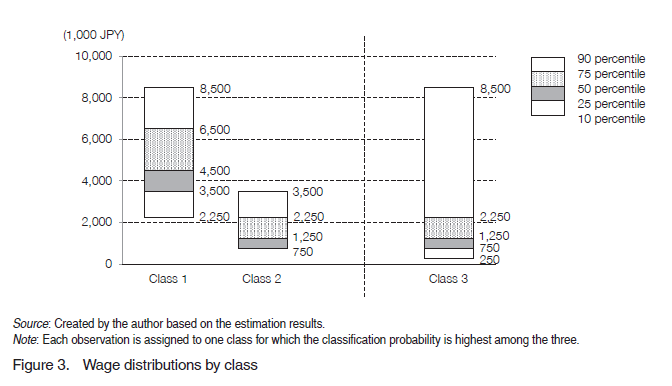
\includegraphics[width=0.85\textheight]{suzuki_perf.png}

\centering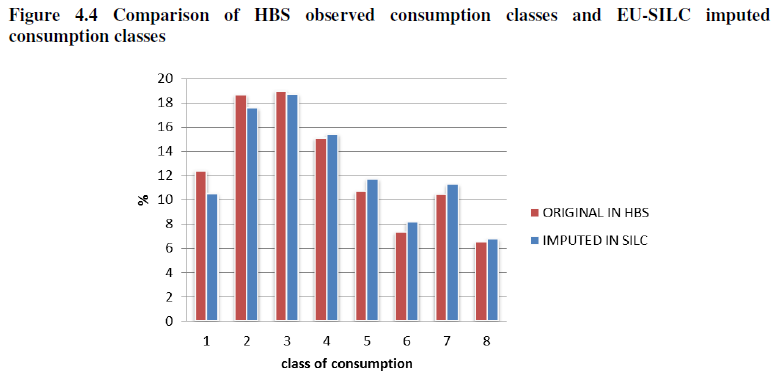
\includegraphics[width=0.85\textheight]{donatiello_perf.png}


\end{frame}



\section{Cierre}

\begin{frame}{Riesgos y limitaciones}
    \small En la entrevista con Germán Rosati, (Doctor en Ciencias Sociales, investigador del CONICET y profesor de la UNSAM), se discutieron los riesgos y limitaciones de la propuesta metodológica. Algunos de los puntos destacados fueron:
    \normalsize
\begin{itemize}
    \item La selección de variables para el clustering es fundamental para la validación de los perfiles encontrados.
    \item La estabilidad de los perfiles encontrados en un momento puntual deben ser asumidos como lo suficientemente estables para ser considerados como perfiles de largo plazo.
\end{itemize}
\end{frame}

\begin{frame}{Expectativas y validaciones}
\begin{enumerate}
    \item Métrica de éxito: replicar tendencia de Lódola/Jaravel con perfiles en vez de deciles
    \item Objetivo: aporte al menú metodológico de la estadística pública de Argentina, con foco en la Ciencia de Datos como herramienta que aporta valor agregado a la investigación económica y sociológica.
\end{enumerate}
\end{frame}

\begin{frame}{¡Gracias!}
\centering\huge¿Preguntas?
\end{frame}

\end{document}
